%% LaTeX-Beamer template for KIT design
%% by Erik Burger, Christian Hammer
%% title picture by Klaus Krogmann
%%
%% version 2.1
%%
%% mostly compatible to KIT corporate design v2.0
%% http://intranet.kit.edu/gestaltungsrichtlinien.php
%%
%% Problems, bugs and comments to
%% burger@kit.edu

\documentclass[18pt]{beamer}

%% SLIDE FORMAT
\setbeamertemplate{navigation symbols}{}

% use 'beamerthemekit' for standard 4:3 ratio
% for widescreen slides (16:9), use 'beamerthemekitwide'
\usepackage[utf8]{inputenc}
\usepackage[T1]{fontenc}
\usepackage{templates/beamerthemekit}
\usepackage{templates/tikzkit}
% \usepackage{templates/beamerthemekitwide}
\usepackage{mathtools}
\usetikzlibrary{chains}

%% TITLE PICTURE

% if a custom picture is to be used on the title page, copy it into the 'logos'
% directory, in the line below, replace 'mypicture' with the 
% filename (without extension) and uncomment the following line
% (picture proportions: 63 : 20 for standard, 169 : 40 for wide
% *.eps format if you use latex+dvips+ps2pdf, 
% *.jpg/*.png/*.pdf if you use pdflatex)

\titleimage{bauplan}

%% TITLE LOGO

% for a custom logo on the front page, copy your file into the 'logos'
% directory, insert the filename in the line below and uncomment it

\titlelogo{plain}

% (*.eps format if you use latex+dvips+ps2pdf,
% *.jpg/*.png/*.pdf if you use pdflatex)

%% TikZ INTEGRATION

% use these packages for PCM symbols and UML classes
% \usepackage{templates/tikzkit}
% \usepackage{templates/tikzuml}

% the presentation starts here

\title[Cellular Graph Automata I]{Cellular Graph Automata I -- Wu \& Rosenfeld}
\subtitle{Zellularautomaten und diskrete komplexe Systeme}
\author{Philipp Faller}
\institute{Thomas Worsch}

% Bibliography

\usepackage[citestyle=authoryear,bibstyle=numeric,hyperref,backend=biber]{biblatex}
\addbibresource{templates/example.bib}
\bibhang1em


\newcommand{\defWord}[1]{\emph{#1}}

\begin{document}

% change the following line to "ngerman" for German style date and logos
\selectlanguage{ngerman}

%title page
\begin{frame}
\titlepage
\end{frame}

%table of contents
% \begin{frame}{Gliederung}
% \tableofcontents
% \end{frame}

\section{$d$"~Graph}
\subsection{Definition}
\begin{frame}{$d$"~Graph}
	\begin{definition}[$d$"~Graph]
		Sei $L$ eine endliche, nicht leere Menge von Beschriftungen mit ausgezeichneten Element $\#$. 
		Ein \defWord{$d$"~Graph} über $L$ ist ein 4"=Tupel $\Gamma = \left(N, A, f, g\right)$, wobei
		\begin{itemize}
			\item[$N$] endliche, nicht leere Menge aus Knoten 
			\item[$A$] $\subseteq N \times N$ symmetrische Relation über $N$ und heißt \defWord{Kantenmenge} von $L$.
			\item[$f$] $: N \rightarrow L$  heißt \defWord{Beschriftungsfunktion}.
			\item[$g$] $: A \rightarrow Z_d$ , mit $Z_d = \left \{1, 2,\text{\dots}, d \right \}$ 			
		\end{itemize}
	\end{definition}
\end{frame}

\begin{frame}{$d$"~Graph}
	\begin{definition}[]
		Weiter muss für $\left(n, m\right) \in A$ gelten:
		\begin{align*}
			f(n) = \# &\implies f(m) \neq \#
		\end{align*}
		
		Sei $A_n := \left \{\left(n, m\right) \in A\right \}$. Dann muss gelten:
		\begin{align*}
			f(n) \neq \# &\implies  \left|A_n\right| = d \text{ und } g \vert_{A_n} \text{ ist Bijektion} \\
			f(n) = \# &\implies\left|A_n\right| = 1
		\end{align*}
		
	\end{definition}
\end{frame}

\subsection{Beispiel}
%\begin{frame}{Beispiel}
%	\centering
%		\begin{tikzpicture}[node distance=2cm, baseline=(current bounding box.north), auto]
%		\node[state](a){$a$};
%		\node[state](c)[below right of=a]{$c$};
%		\node[state](b)[above right of=c]{$b$};
%		\foreach \q/\p/\a/\b in {a/b/1/1, a/c/2/1, b/c/2/2}
%		\draw[->] (\q) edge[bend left=9] node {\a} (\p) 
%		(\p) edge[bend left=9] node {\b} (\q) 
%		;
%		
%		\end{tikzpicture}
%\end{frame}


\begin{frame}{Beispiel}
	\centering
		\begin{tikzpicture}[node distance=2cm, baseline=(current bounding box.north), auto]
		\node[state](a){$a$};
		\node[state](b)[right of = a]{$b$};
		\node[state](d)[right of = b]{$d$};
		\node[state](f)[below right of = d]{$f$};
		\node[state](e)[below left of = f]{$e$};
		\node[state](c)[left of = e]{$c$};
		\node[state](a1)[left of = a]{$\#$};
		\node[state](c1)[left of = c]{$\#$};
		\node[state](a2)[left of = c1]{$\#$};
		\node[state](f1)[right of = f]{$\#$};
		
		
		\foreach \p/\q/\a/\b in {a/b/1/2, b/d/1/2, b/c/2/3, d/e/2/3, d/f/1/2, e/f/3/3, c/e/1/3, a1/a/1/1, a2/a/3/1, c1/c/1/1, f1/f/2/1}
		\draw[->] 
		(\q) edge[bend left=9] node {\a} (\p) 
		(\p) edge[bend left=9] node {\b} (\q) 			
		;
		\end{tikzpicture}
\end{frame}

\subsection{Weitere Definitionen}
\begin{frame}{Zugrunde liegender Graph}
	\begin{definition}[Zugrunde liegender Graph]
		Sei $\Gamma$ ein $d$"~Graph. 
		Der Graph $G(\Gamma) = \left(V, E\right)$ mit
		\begin{align*}
			V &= N\setminus \left\{n \in N \mid f\left(n\right) = \# \right\} \\		
			E &= A\setminus \left\{\left(n, m\right) \in A \mid f(n) = \# \lor f(m) = \# \right\}
		\end{align*} 
		heißt der \defWord{$\Gamma$ zugrunde liegende Graph}.
	\end{definition}
	\begin{definition}[Zusammenhängend]
		Ein $d$"~Graph heißt \defWord{zusammenhängend}, wenn der zugrunde liegende Graph zusammenhängend ist.
	\end{definition}
\end{frame}

%TODO Unnötige Folie?
\begin{frame}{Nachbarschaft}
	\begin{definition}[Nachbarschaft]
		Sei $\left(n, m\right) \in A$ und $g\left(n, m\right) = i$. 
		Dann heißt $m$ der \defWord{$i$"=te Nachbar von $n$}.
		Außerdem gilt: 
		\begin{displaymath}
		\left(m, n\right) \in A \text{ und }\exists j \in Z_d : g(m, n) = j.
		\end{displaymath}
		Dann ist $n$ der $j$"=te Nachbar von $m$. 
		Definiere $h : N \times Z_d \rightarrow N$, so dass
		\begin{displaymath}
		h(n, i) = m \iff g(n, m) = i.
		\end{displaymath}
	\end{definition}
\end{frame}

\section{Zellulare $d$"~Graph Automaten}
\subsection{Definition}
\begin{frame}{Zellulare $d$"~Graph Automaten}
	\begin{definition}[$d$"~Graph Automat]
		Ein \defWord{Zellulärer $d$"~Graph Automat} $\mathcal{M}$ ist ein Tripel $\left(\Gamma, M, H\right)$, wobei
		\begin{itemize}
			\item[$\Gamma$] ein $d$"~Graph $\left(N, A, f, g\right)$ über Menge von Beschriftungen $L$
			\item[$M$] endlicher Automat $\left(Q, \delta\right)$, mit 
			\begin{itemize}
				\item[$Q$] endliche, nicht leere Menge von Zuständen, mit $L \subseteq Q$.
				\item[$\delta$] $\cramped{: Q \times Z_d^d \times Q^d \rightarrow \mathcal{P}\left(Q\right)}$  heißt \defWord{Zustandsübergangsfunktion}.
				
				Dabei ist $\cramped{\delta(\#, z, q) = \{\# \}}, \forall z \in Z_d^d, q \in Q^d$
			\end{itemize}
			\item[$H$] $: N \rightarrow Z_d^d$. 
			Für $n \in N$ heißt $H(n) = \left(t_1, \text{\dots}, t_n\right) \in Z_d^d$ \defWord{Nachbarschaftsvektor} von $n$. 
		\end{itemize}
	\end{definition}
\end{frame}
\begin{frame}{Zellulare $d$"~Graph Automaten}
	\begin{columns}
		\begin{column}{0.48\textwidth}
		\centering
		\begin{tikzpicture}[node distance=2cm, baseline=(current bounding box.north), auto]
		\node[state](a){$a$};
		\node[state](c)[below right of=a]{$c$};
		\node[state](b)[above right of=c]{$b$};
		\foreach \q/\p/\a/\b in {a/b/1/1, a/c/2/1, b/c/2/2}
		\draw[->] (\q) edge[bend left=9] node {\a} (\p) 
		(\p) edge[bend left=9] node {\b} (\q) 
		;
		
		\end{tikzpicture}
		\end{column}
		\begin{column}{0.48\textwidth}
			\begin{itemize}
				\item H(a) = (1, 1)
				\item H(b) = (1, 2)
				\item H(c) = (2, 2)
			\end{itemize}
		\end{column}
	\end{columns}
	
\end{frame}

\begin{frame}{Zellulare $d$"~Graph Automaten}
	\begin{definition}[Konfiguration]
		Eine \defWord{Konfiguration von $\mathcal{M}$} ist eine Abbildung \hbox{$c : N \rightarrow Q$}.
		
		Sei $n$ ein Knoten mit Nachbarn $m_1, \dots, m_d$		
		und $q_m = \left( c(m_1), \dots , c(m_d)\right) \in Q^d$. 
		Der Folgezustand $c'(n)$ des Knotens $n$ ist dann gegeben durch 
		\begin{displaymath}
		c'(n) = \delta(c(n), H(n),q_m ).
		\end{displaymath} 
		Wir sagen $\delta$ überführt $c$ in $c'$ und schreiben $c \vdash c'$.
	\end{definition}
\end{frame}

\begin{frame}{Zellulare $d$"~Graph Automaten}
	\begin{exampleblock}{Bemerkung}
		Der Zellulare $d$"~Graph Automat ist eine Verallgemeinerung des \emph{endlichen} Zellularautomaten.
	\end{exampleblock}
	\centering
	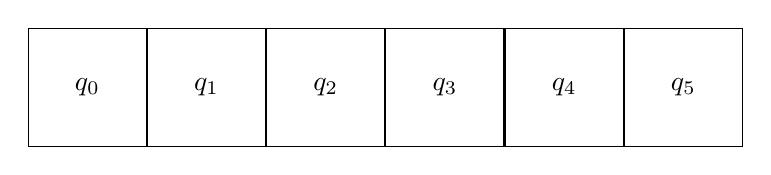
\begin{tikzpicture}[node distance=2cm, baseline=(current bounding box.north)]
	
	\begin{scope}[start chain=1 going right,node distance=0cm]
	\node[on chain=1, draw, minimum size = 1.5cm] (a){$q_0$};
	\node[on chain=1, draw, minimum size = 1.5cm] (b){$q_1$};
	\node[on chain=1, draw, minimum size = 1.5cm] (c) {$q_2$};
	\node[on chain=1, draw, minimum size = 1.5cm]  (d) {$q_3$};
	\node[on chain=1, draw, minimum size = 1.5cm]  (e) {$q_4$};
	\node[on chain=1, draw, minimum size = 1.5cm]  (f) {$q_5$};
	\end{scope}
	
	
	\end{tikzpicture}
	
	\vspace{0.75cm}
	\begin{tikzpicture}[node distance=1.5cm, baseline=(current bounding box.north), every state/.style={minimum size = 3.3em}]
	\node[state] (a) {$q_5$};
	\node[state] (b)[left of = a] {$q_4$};
	\node[state] (c)[left of = b] {$q_3$};
	\node[state] (d)[left of = c] {$q_2$};
	\node[state] (e)[left of = d] {$q_1$};
	\node[state] (f)[left of = e] {$q_0$};
	\node[state] (a1)[right of = a] {$\#$};
	\node[state] (f1)[left of = f] {$\#$};
	
	\foreach \p/\q in {a/b, b/c, c/d, d/e, e/f, a/a1, f/f1}
	\draw[->] 
	(\q) edge (\p)
	(\p) edge (\q) 			
	;
	\end{tikzpicture}
		
\end{frame}

\definecolor{S3}{named}{kit-green100}
\definecolor{S1}{named}{kit-blue100}
\definecolor{S2}{named}{kit-red70}
%TODO Sprachen
\section{Spannbaum durch Breitensuche}
\subsection{Algorithmus}
\begin{frame}{Spannbaum durch Breitensuche}
	
	Wir bestimmen einen Spannbaum von minimaler Höhe zur Wurzel $k$.
	\begin{itemize}
		\item Wurzel $k$ sendet Signal $S$ aus.
		\item Erhält Knoten $n$ zum erste Mal $S$ (von einem Knoten $m$), ist $m$ der Vater von $n$. Falls mehrere gleichzeitig senden, wähle einen beliebigen Knoten als Vater aus.
		\item $m$ sendet $S$ weiter und zeigt an, dass $n$ sein Vater ist. Dann weiß $n$, dass $m$ sein Kind ist.
		\item Ein Blatt sendet $S'$ aus, sobald feststeht, dass es eines ist. 
		\item $S'$ wird von einem Knoten $n$ weitergeleitet, wenn alle Kinder von $n$ das Signal $S'$ gesendet haben.
	\end{itemize}
	$\implies 2r(k) \text{ Schritte}$
\end{frame}

\subsection{Beispiel}
\begin{frame}{Spannbaum durch Breitensuche}
	\centering
	\begin{overprint}
	\only<+>{
		\begin{tikzpicture}[node distance=2cm, baseline=(current bounding box.mid), every state/.style={minimum size = 3.3em}]
			\node[state](a){$a$};
			\node[state, fill=S2, accepting](b)[right of = a]{$b$};
			\node[state](d)[right of = b]{$d$};
			\node[state](f)[below right of = d]{$f$};
			\node[state](e)[below left of = f]{$e$};
			\node[state](c)[left of = e]{$c$};
			\node[state](a1)[left of = a]{$\#$};
			\node[state](a2)[below left of = a]{$\#$};
			\node[state](c1)[left of = c]{$\#$};
			\node[state](f1)[right of = f]{$\#$};
	
			\foreach \p/\q in {a/b, b/d, b/c, d/e, d/f, e/f, c/e, a1/a, a2/a, c1/c, f1/f}
			\draw[->] 
			(\q) edge[bend left=9] (\p)
			(\p) edge[bend left=9] (\q) 			
			;
		\end{tikzpicture}
	}
	\only<+>{
		\begin{tikzpicture}[node distance=2cm, baseline=(current bounding box.mid), every state/.style={minimum size = 3.3em}]
		\node[state, fill=S2](a){$a$};
		\node[state, fill=S1, text=white, accepting](b)[right of = a]{$b$};
		\node[state, fill=S2](d)[right of = b]{$d$};
		\node[state](f)[below right of = d]{$f$};
		\node[state](e)[below left of = f]{$e$};
		\node[state, fill=S2](c)[left of = e]{$c$};
		\node[state](a1)[left of = a]{$\#$};
		\node[state](a2)[below left of = a]{$\#$};
		\node[state](c1)[left of = c]{$\#$};
		\node[state](f1)[right of = f]{$\#$};
		
		
		\foreach \p/\q in {a/b, b/d, b/c, d/e, d/f, e/f, c/e, a1/a, a2/a, c1/c, f1/f}
		\draw[->] 
		(\q) edge[bend left=9] (\p)
		(\p) edge[bend left=9] (\q) 			
		;
		\foreach \p/\q in {a/b, d/b, c/b}
		\draw[->] 
		(\p) edge[bend left=9, line width = 2pt, S1] (\q) 			
		;		
		\end{tikzpicture}
	}
	\only<+>{
		\begin{tikzpicture}[node distance=2cm, baseline=(current bounding box.mid), every state/.style={minimum size = 3.3em}]
		\node[state, fill=S3, text=white](a){$a$};
		\node[state, fill=S1, text=white, accepting](b)[right of = a]{$b$};
		\node[state, fill=S1, text=white](d)[right of = b]{$d$};
		\node[state, fill=S2](f)[below right of = d]{$f$};
		\node[state, fill=S2](e)[below left of = f]{$e$};
		\node[state, fill=S1, text=white](c)[left of = e]{$c$};
		\node[state](a1)[left of = a]{$\#$};
		\node[state](a2)[below left of = a]{$\#$};
		\node[state](c1)[left of = c]{$\#$};
		\node[state](f1)[right of = f]{$\#$};
		
		\foreach \p/\q in {a/b, b/d, b/c, d/e, d/f, e/f, c/e, a1/a, a2/a, c1/c, f1/f}
		\draw[->] 
		(\q) edge[bend left=9] (\p)
		(\p) edge[bend left=9] (\q) 			
		;
		\foreach \p/\q in {a/b, d/b, c/b, e/d, f/d}
		\draw[->] 
		(\p) edge[bend left=9, line width = 2pt, S1] (\q) 			
		;
		\foreach \p/\q in {b/a, b/c, b/d}
		\draw[->] 
		(\p) edge[bend left=9, line width = 2pt, S3] (\q) 			
		;	
		
		\end{tikzpicture}
	}
	\only<+>{
		\begin{tikzpicture}[node distance=2cm, baseline=(current bounding box.mid), every state/.style={minimum size = 3.3em}]
		\node[state, fill=S3, text=white](a){$a$};
		\node[state, fill=S1, text=white, accepting](b)[right of = a]{$b$};
		\node[state, fill=S1, text=white](d)[right of = b]{$d$};
		\node[state, fill=S3, text=white](f)[below right of = d]{$f$};
		\node[state, fill=S3, text=white](e)[below left of = f]{$e$};
		\node[state, fill=S3, text=white](c)[left of = e]{$c$};
		\node[state](a1)[left of = a]{$\#$};
		\node[state](a2)[below left of = a]{$\#$};
		\node[state](c1)[left of = c]{$\#$};
		\node[state](f1)[right of = f]{$\#$};
		
		\foreach \p/\q in {a/b, b/d, b/c, d/e, d/f, e/f, c/e, a1/a, a2/a, c1/c, f1/f}
		\draw[->] 
		(\q) edge[bend left=9] (\p)
		(\p) edge[bend left=9] (\q) 			
		;
		\foreach \p/\q in {a/b, d/b, c/b, e/d, f/d}
		\draw[->] 
		(\p) edge[bend left=9, line width = 2pt, S1] (\q) 			
		;	
		\foreach \p/\q in {b/a, b/c, b/d, d/e, d/f}
		\draw[->] 
		(\p) edge[bend left=9, line width = 2pt, S3] (\q) 			
		;	
		\end{tikzpicture}
	}
	\only<+>{
		\begin{tikzpicture}[node distance=2cm, baseline=(current bounding box.mid), every state/.style={minimum size = 3.3em}]
		\node[state, fill=S3, text=white](a){$a$};
		\node[state, fill=S1, text=white, accepting](b)[right of = a]{$b$};
		\node[state, fill=S3, text=white](d)[right of = b]{$d$};
		\node[state, fill=S3, text=white](f)[below right of = d]{$f$};
		\node[state, fill=S3, text=white](e)[below left of = f]{$e$};
		\node[state, fill=S3, text=white](c)[left of = e]{$c$};
		\node[state](a1)[left of = a]{$\#$};
		\node[state](a2)[below left of = a]{$\#$};
		\node[state](c1)[left of = c]{$\#$};
		\node[state](f1)[right of = f]{$\#$};
		
		\foreach \p/\q in {a/b, b/d, b/c, d/e, d/f, e/f, c/e, a1/a, a2/a, c1/c, f1/f}
		\draw[->] 
		(\q) edge[bend left=9] (\p)
		(\p) edge[bend left=9] (\q) 			
		;
		\foreach \p/\q in {a/b, d/b, c/b, e/d, f/d}
		\draw[->] 
		(\p) edge[bend left=9, line width = 2pt, S1] (\q) 			
		;	
		\foreach \p/\q in {b/a, b/c, b/d, d/e, d/f}
		\draw[->] 
		(\p) edge[bend left=9, line width = 2pt, S3] (\q) 			
		;	
		\end{tikzpicture}
	}
	\only<+>{
		\begin{tikzpicture}[node distance=2cm, baseline=(current bounding box.mid), every state/.style={minimum size = 3.3em}]
		\node[state, fill=S3, text=white](a){$a$};
		\node[state, fill=S3, text=white, accepting](b)[right of = a]{$b$};
		\node[state, fill=S3, text=white](d)[right of = b]{$d$};
		\node[state, fill=S3, text=white](f)[below right of = d]{$f$};
		\node[state, fill=S3, text=white](e)[below left of = f]{$e$};
		\node[state, fill=S3, text=white](c)[left of = e]{$c$};
		\node[state](a1)[left of = a]{$\#$};
		\node[state](a2)[below left of = a]{$\#$};
		\node[state](c1)[left of = c]{$\#$};
		\node[state](f1)[right of = f]{$\#$};
		
		
		\foreach \p/\q in {a/b, b/d, b/c, d/e, d/f, e/f, c/e, a1/a, a2/a, c1/c, f1/f}
		\draw[->] 
		(\q) edge[bend left=9] (\p)
		(\p) edge[bend left=9] (\q) 			
		;
		\foreach \p/\q in {a/b, d/b, c/b, e/d, f/d}
		\draw[->] 
		(\p) edge[bend left=9, line width = 2pt, S1] (\q) 			
		;
		\foreach \p/\q in {b/a, b/c, b/d, d/e, d/f}
		\draw[->] 
		(\p) edge[bend left=9, line width = 2pt, S3] (\q) 			
		;
		\end{tikzpicture}
	}
	\only<+>{
		\begin{tikzpicture}[node distance=2cm, baseline=(current bounding box.mid), every state/.style={minimum size = 3.3em}]
		\node[state, accepting, fill=S3, text=white](b){$b$};
		\node[state, fill=S3, text=white](c)[below of = b]{$c$};
		\node[state, fill=S3, text=white](d)[right of = c]{$d$};
		\node[state, fill=S3, text=white](a)[left of = c]{$a$};
%		\node[state](a1)[below of = a]{$\#$};
%		\node[state](a2)[left of = a1]{$\#$};
%		\node[state](c1)[below of = c]{$\#$};
		\node[state, fill=S3, text=white](e)[below of = d]{$e$};
		\node[state, fill=S3, text=white](f)[right of = e]{$f$};
%		\node[state](f1)[below of = f]{$\#$};
		
		
		\foreach \p/\q in {a/b, b/d, b/c, d/e, d/f}
		\draw[->] 
		(\q) edge[bend left=9] (\p)
		(\p) edge[bend left=9] (\q) 			
		;
		\foreach \p/\q in {a/b, d/b, c/b, e/d, f/d}
		\draw[->] 
		(\p) edge[bend left=9, line width = 2pt, S1] (\q) 			
		;
		\foreach \p/\q in {b/a, b/c, b/d, d/e, d/f}
		\draw[->] 
		(\p) edge[bend left=9, line width = 2pt, S3] (\q) 			
		;
		
		\end{tikzpicture}
	}			
		\end{overprint}
\end{frame}
\section{Radius bestimmen}
\subsection{Definition}
\begin{frame}{Radius bestimmen}
	\begin{definition}[Abstand]
		Sei $\Gamma$ ein zusammenhängender $d$"~Graph, $k$ ein Knoten von $\Gamma$ mit $f\left(k\right) \neq \#$.
		Der \defWord{Abstand zwischen zwei Knoten $m, n$ in $\Gamma$}, geschrieben $\text{dist}\left(m , n\right)$, ist die Länge des kürzesten Weges von $m$ nach $n$.
	\end{definition}
	\begin{definition}[Radius]
		Weiter heißt
		\begin{displaymath}
			r\left(k\right) := \max_{\mathclap{f\left(n\right) \neq \#}} \text{ dist}\left(k, n\right)
		\end{displaymath}
		der \defWord{Radius von $\Gamma$ vom Zentrum $k$ aus}.
	\end{definition}
\end{frame}
\subsection{Algorithmus}
\begin{frame}{Radius bestimmen}
	\begin{exampleblock}{Bemerkung}
		Sei $T$ ein Spannbaum mit Wurzel $k$ und Höhe $h$, wie im letzten Abschnitt. Da $T$ durch Breitensuche konstruiert wurde, sind die Äste kürzeste Wege und es gilt:
		\begin{displaymath}
			h = \max_{\mathclap{f\left(n\right) \neq \#}} \text{ dist}\left(k, n\right) = r(k)
		\end{displaymath}
		
		Die Höhe von $T$ kann im Längsten Ast binär gespeichert werden, da
		\begin{displaymath}
			h < 2^{h + 1} , \forall h \in \mathbb{N}
		\end{displaymath}
	\end{exampleblock}
\end{frame}

\begin{frame}{Radius bestimmen}
	Wir bestimmen den Radius des Knotens $k$.
	\begin{itemize}
		\item Spannbaum mit Wurzel $k$ erzeugen.
		\item Sende Signal $S_1$ von $k$ aus.
		\item Erhält ein Blatt das Signal $S_1$, sendet es Signal $S_2$ zu seinem Elternknoten.
		\item Hat ein Knoten $m$ das Signal $S_2$ von einem Kind $m_1$ erhalten, aber noch nicht von einem anderen Kind $m_2$, sendet $m$ ein Signal $R$ zu $m_1$.
		\item Erhält $k$ das Signal $S_2$ von seinem letzten Kind, sendet $k$ Signal $S_3$ entlang des Astes.
		\item Das Blatt des Astes sendet $S_3'$ zurück.
		\item Zähle Länge des Astes. 
	\end{itemize}
	$\implies 2r(k) + 4r(k) = 6r(k) \text{ Schritte}$
\end{frame}

\begin{frame}{Radius bestimmen}
	Um die Länge des Astes zu bestimmen gehen wir folgendermaßen vor:
	
	Jeder Knoten speichert ein Zählerbit und ein Carrybit.
	\begin{itemize}
		\item $k$ sendet Signal $S_1$ aus und erhöht Zähler um 1. 
		\item Jeden zweiten Zeitschritt wird der Zähler von $k$ inkrementiert.
		\item Ist das Carrybit gesetzt, übernimmt das Kind dieses in seinen Zähler.
		\item Erhält das Blatt das Signal $S_1$ sendet es $S_1'$ zurück.
		\item Erhält $k$ das Signal $S_1'$ stoppt $k$ das inkrementieren.
		\item $k$ sendet noch ein Signal $S_2$ den Ast entlang.
		\item Das Blatt sendet $S_2'$ zurück.
	\end{itemize}
	$\implies 6r(k) + 4r(k) = 10r(k) \text{ Schritte}$
\end{frame}

\subsection{Beispiel}
\definecolor{S}{named}{kit-green100}
\begin{frame}{Radius bestimmen}
	
	\centering
	\begin{overprint}	
	\only<1>{
	\begin{tikzpicture}[node distance=2cm, baseline=(current bounding box.north)]
	\node[state, accepting] (a) {$0\mid 0$};
	\node[state] (b)[left of = a] {$0\mid 0$};
	\node[state] (c)[left of = b] {$0\mid 0$};
	\node[state] (d)[left of = c] {$0\mid 0$};
	\node[state] (e)[left of = d] {$0\mid 0$};
	\node[state] (f)[left of = e] {$0\mid 0$};
	
	\foreach \p/\q in {a/b, b/c, c/d, d/e, e/f}
	\draw[->] 
	(\q) edge (\p)
	(\p) edge (\q) 			
	;
	\end{tikzpicture}		
	}
	\only<1-2>{	
	\begin{tikzpicture}[node distance=2cm, baseline=(current bounding box.north)]
	\node[state, fill=S, text=white, accepting] (a) {$0\mid 1$};
	\node[state] (b)[left of = a] {$0\mid 0$};
	\node[state] (c)[left of = b] {$0\mid 0$};
	\node[state] (d)[left of = c] {$0\mid 0$};
	\node[state] (e)[left of = d] {$0\mid 0$};
	\node[state] (f)[left of = e] {$0\mid 0$};
	
	\foreach \p/\q in {a/b, b/c, c/d, d/e, e/f}
	\draw[->] 
	(\q) edge (\p)
	(\p) edge (\q) 			
	;
	\end{tikzpicture}
	}
	\only<1-3>{	
	\begin{tikzpicture}[node distance=2cm, baseline=(current bounding box.north)]
	\node[state, accepting] (a) {$0\mid 1$};
	\node[state, fill=S, text=white] (b)[left of = a] {$0\mid 0$};
	\node[state] (c)[left of = b] {$0\mid 0$};
	\node[state] (d)[left of = c] {$0\mid 0$};
	\node[state] (e)[left of = d] {$0\mid 0$};
	\node[state] (f)[left of = e] {$0\mid 0$};
	
	\foreach \p/\q in {a/b, b/c, c/d, d/e, e/f}
	\draw[->] 
	(\q) edge (\p)
	(\p) edge (\q) 			
	;
	\end{tikzpicture}
	}
	\only<1-4>{	
	\begin{tikzpicture}[node distance=2cm, baseline=(current bounding box.north)]
	\node[state, accepting] (a) {$1\mid 0$};
	\node[state] (b)[left of = a] {$0\mid 0$};
	\node[state, fill=S, text=white] (c)[left of = b] {$0\mid 0$};
	\node[state] (d)[left of = c] {$0\mid 0$};
	\node[state] (e)[left of = d] {$0\mid 0$};
	\node[state] (f)[left of = e] {$0\mid 0$};
	
	\foreach \p/\q in {a/b, b/c, c/d, d/e, e/f}
	\draw[->] 
	(\q) edge (\p)
	(\p) edge (\q) 			
	;
	\end{tikzpicture}
	}
	\only<1-5>{	
	\begin{tikzpicture}[node distance=2cm, baseline=(current bounding box.north)]
	\node[state, accepting] (a) {$0\mid 0$};
	\node[state] (b)[left of = a] {$0\mid 1$};
	\node[state] (c)[left of = b] {$0\mid 0$};
	\node[state, fill=S, text=white] (d)[left of = c] {$0\mid 0$};
	\node[state] (e)[left of = d] {$0\mid 0$};
	\node[state] (f)[left of = e] {$0\mid 0$};
	
	\foreach \p/\q in {a/b, b/c, c/d, d/e, e/f}
	\draw[->] 
	(\q) edge (\p)
	(\p) edge (\q) 			
	;
	\end{tikzpicture}
	}
	\only<1-6>{	
	\begin{tikzpicture}[node distance=2cm, baseline=(current bounding box.north)]
	\node[state, accepting] (a) {$0\mid 1$};
	\node[state] (b)[left of = a] {$0\mid 1$};
	\node[state] (c)[left of = b] {$0\mid 0$};
	\node[state] (d)[left of = c] {$0\mid 0$};
	\node[state, fill=S, text=white] (e)[left of = d] {$0\mid 0$};
	\node[state] (f)[left of = e] {$0\mid 0$};
	
	\foreach \p/\q in {a/b, b/c, c/d, d/e, e/f}
	\draw[->] 
	(\q) edge (\p)
	(\p) edge (\q) 			
	;
	\end{tikzpicture}
	}
	\only<2->{	
	\begin{tikzpicture}[node distance=2cm, baseline=(current bounding box.north)]
	\node[state, accepting] (a) {$0\mid 1$};
	\node[state] (b)[left of = a] {$0\mid 1$};
	\node[state] (c)[left of = b] {$0\mid 0$};
	\node[state] (d)[left of = c] {$0\mid 0$};
	\node[state] (e)[left of = d] {$0\mid 0$};
	\node[state, fill=S, text=white] (f)[left of = e] {$0\mid 0$};
	
	\foreach \p/\q in {a/b, b/c, c/d, d/e, e/f}
	\draw[->] 
	(\q) edge (\p)
	(\p) edge (\q) 			
	;
	\end{tikzpicture}
	}
	\only<3->{	
	\begin{tikzpicture}[node distance=2cm, baseline=(current bounding box.north)]
	\node[state, accepting] (a) {$1\mid 0$};
	\node[state] (b)[left of = a] {$0\mid 1$};
	\node[state] (c)[left of = b] {$0\mid 0$};
	\node[state] (d)[left of = c] {$0\mid 0$};
	\node[state, fill=S, text=white] (e)[left of = d] {$0\mid 0$};
	\node[state] (f)[left of = e] {$0\mid 0$};
	
	\foreach \p/\q in {a/b, b/c, c/d, d/e, e/f}
	\draw[->] 
	(\q) edge (\p)
	(\p) edge (\q) 			
	;
	\end{tikzpicture}
	}
	\only<4->{	
	\begin{tikzpicture}[node distance=2cm, baseline=(current bounding box.north)]
	\node[state, accepting] (a) {$0\mid 0$};
	\node[state] (b)[left of = a] {$1\mid 0$};
	\node[state] (c)[left of = b] {$0\mid 0$};
	\node[state, fill=S, text=white] (d)[left of = c] {$0\mid 0$};
	\node[state] (e)[left of = d] {$0\mid 0$};
	\node[state] (f)[left of = e] {$0\mid 0$};
	
	\foreach \p/\q in {a/b, b/c, c/d, d/e, e/f}
	\draw[->] 
	(\q) edge (\p)
	(\p) edge (\q) 			
	;
	\end{tikzpicture}
	}
	\only<5->{	
	\begin{tikzpicture}[node distance=2cm, baseline=(current bounding box.north)]
	\node[state, accepting] (a) {$0\mid 1$};
	\node[state] (b)[left of = a] {$0\mid 0$};
	\node[state, fill=S, text=white] (c)[left of = b] {$0\mid 1$};
	\node[state] (d)[left of = c] {$0\mid 0$};
	\node[state] (e)[left of = d] {$0\mid 0$};
	\node[state] (f)[left of = e] {$0\mid 0$};
	
	\foreach \p/\q in {a/b, b/c, c/d, d/e, e/f}
	\draw[->] 
	(\q) edge (\p)
	(\p) edge (\q) 			
	;
	\end{tikzpicture}
	}
	\only<6->{	
	\begin{tikzpicture}[node distance=2cm, baseline=(current bounding box.north)]
	\node[state, accepting] (a) {$0\mid 1$};
	\node[state, fill=S, text=white] (b)[left of = a] {$0\mid 0$};
	\node[state] (c)[left of = b] {$0\mid 1$};
	\node[state] (d)[left of = c] {$0\mid 0$};
	\node[state] (e)[left of = d] {$0\mid 0$};
	\node[state] (f)[left of = e] {$0\mid 0$};
	
	\foreach \p/\q in {a/b, b/c, c/d, d/e, e/f}
	\draw[->] 
	(\q) edge (\p)
	(\p) edge (\q) 			
	;
	\end{tikzpicture}
	}
	\only<7->{	
	\begin{tikzpicture}[node distance=2cm, baseline=(current bounding box.north)]
	\node[state, fill=S, text=white, accepting] (a) {$0\mid 1$};
	\node[state] (b)[left of = a] {$0\mid 0$};
	\node[state] (c)[left of = b] {$0\mid 1$};
	\node[state] (d)[left of = c] {$0\mid 0$};
	\node[state] (e)[left of = d] {$0\mid 0$};
	\node[state] (f)[left of = e] {$0\mid 0$};
	
	\foreach \p/\q in {a/b, b/c, c/d, d/e, e/f}
	\draw[->] 
	(\q) edge (\p)
	(\p) edge (\q) 			
	;
	\end{tikzpicture}
	}	
	\end{overprint}
\end{frame}

\section{Zellulare $d$"~Graph Akzeptoren}
\subsection{Definition}
\begin{frame}{Zellularer $d$"~Graph Akzeptor}
	\begin{definition}[Ausgezeichneter Knoten]
		Ein $d$"~Graph Automat, bei dem genau ein Knoten eine Marke als Teil seines Zustandes  besitzt, heißt \defWord{Zellularer $d$"~Graph Automat mit ausgezeichnetem Knoten}.
	\end{definition}
	\begin{definition}[Zellularer $d$"~Graph Akzeptor]
		Sei $\mathcal{M} = \left(\Gamma, (Q, \delta), H \right)$ ein $d$"~Graph Automat mit ausgezeichnetem Knoten , sodass $(L, Q, \delta, F)$ ein endlicher Akzeptor ist.
		Dann heißt $\mathcal{M}$ \defWord{Zellularer $d$"~Graph Akzeptor}.
	\end{definition}
\end{frame}

\begin{frame}{Sprache}
	\begin{definition}[Akzeptanz]
		Ein $d$"~Graph Akzeptor \defWord{akzeptiert} $\Gamma$, wenn es eine endliche Folge von Konfigurationen $\left(c_i\right)_{1 \le i \le m}$ gibt, mit
		\begin{displaymath}
		c_1 = f, c_m(\hat{n}) \in F
		\end{displaymath}
		für den ausgezeichneten Knoten $\hat{n}$, sodass:
		\begin{displaymath}
		c_{i} \vdash c_{i+1} \text{, für } 1 \le i \le m
		\end{displaymath}
	\end{definition}
	\begin{definition}[Sprache]
		Die \defWord{Sprache von $d$"=Graphen, die durch $M$ akzeptiert wird} ist die Menge 
		\begin{displaymath}
		\mathcal{L}(M) = \left\{\Gamma \mid \mathcal{M} = \left(\Gamma, M, H\right) \text{ akzeptiert } \Gamma \right\}
		\end{displaymath}
	\end{definition}
\end{frame}
\subsection{Beispiel}

\definecolor{S3}{named}{kit-green100}
\definecolor{S1}{named}{kit-blue100}
\definecolor{S2}{named}{kit-red70}
\begin{frame}{Beispiel}
	$\mathcal{L}(M) = \{\Gamma \mid \text{Der $\Gamma$ zugrunde liegende Graph ist bipartit}\}$
	\centering{
	\begin{overprint}
		\only<+>{	
			\begin{tikzpicture}[node distance=2cm, baseline=(current bounding box.north)]
			\node[state, accepting, fill=S1] (a) {};
			\node[state] (b)[below of = a] {};
			\node[state] (c)[below of = b] {};
			\node[state] (d)[right of = a] {};
			\node[state] (e)[below of = d] {};
			\node[state] (f)[below of = e] {};
			
			\foreach \p/\q in {a/d, a/e, a/f, b/d, b/e, b/f, c/d, c/e, c/f}
			\draw[->] 
			(\q) edge (\p)
			(\p) edge (\q) 			
			;
			\end{tikzpicture}
		}
		\only<+>{	
			\begin{tikzpicture}[node distance=2cm, baseline=(current bounding box.north)]
			\node[state, accepting, fill=S1] (a) {};
			\node[state] (b)[below of = a] {};
			\node[state] (c)[below of = b] {};
			\node[state, fill=S3] (d)[right of = a] {};
			\node[state, fill=S3] (e)[below of = d] {};
			\node[state, fill=S3] (f)[below of = e] {};
			
			\foreach \p/\q in {a/d, a/e, a/f, b/d, b/e, b/f, c/d, c/e, c/f}
			\draw[->] 
			(\q) edge (\p)
			(\p) edge (\q) 			
			;
			\end{tikzpicture}
		}
		\only<+>{	
			\begin{tikzpicture}[node distance=2cm, baseline=(current bounding box.north)]
			\node[state, accepting, fill=S1] (a) {};
			\node[state, fill=S1] (b)[below of = a] {};
			\node[state, fill=S1] (c)[below of = b] {};
			\node[state, fill=S3] (d)[right of = a] {};
			\node[state, fill=S3] (e)[below of = d] {};
			\node[state, fill=S3] (f)[below of = e] {};
			
			\foreach \p/\q in {a/d, a/e, a/f, b/d, b/e, b/f, c/d, c/e, c/f}
			\draw[->] 
			(\q) edge (\p)
			(\p) edge (\q) 			
			;
			\end{tikzpicture}
		}	
	\end{overprint}
}
\end{frame}
\end{document}
